\documentclass{article}
\usepackage{color}
\usepackage{tikz}
\usepackage{pgfplotstable}
\usepackage{chngcntr}
\usepackage[toc,page,title]{appendix}
\usepackage{float}
\usepackage{tabularx}
\usepackage{amsmath}
\usepackage{amssymb}
\usepackage{listings}
\usepackage{enumitem}
\usepackage{syntax}
\usepackage{csquotes}
\usepackage{pgfplots}
\usepackage[backend=biber]{biblatex}
\addbibresource{references.bib}

\usetikzlibrary{matrix}

\definecolor{dkgreen}{rgb}{0,0.6,0}
\definecolor{gray}{rgb}{0.5,0.5,0.5}
\definecolor{mauve}{rgb}{0.58,0,0.82}
\definecolor{variables}{RGB}{126,25,121}
\definecolor{symbolred}{RGB}{178,34,34}


\lstdefinelanguage{eprime}
{
	morekeywords={
		letting, be,
		indexed, by, of,
		given, 
		find,
		maximising, minimising,
		such, that,
		max, min,
		sum,
		forall, forAll, exists, alldifferent, table
	},
	morecomment=[l]{\$},
}

\lstset{
  language={eprime},
  frame=tb,
  alsoletter={\\}!.:+\=-<>{/}{..},
  emph = [1]{int, bool, matrix, domain},
  emphstyle = [1]{\color{variables}},
  emph = [2]{:, !=, ->, \=, +, -, ., .., *, \%, /\\, \\/, <, >, =},
  emphstyle = [2]{\color{symbolred}},  
  numbers=left,
  stepnumber=1,
  aboveskip=3mm,
  belowskip=3mm,
  showstringspaces=false,
  columns=flexible,
  basicstyle={\small\ttfamily},
  numberstyle=\color{gray},
  keywordstyle=\color{blue},
  commentstyle=\color{dkgreen},
  stringstyle=\color{mauve},
  breaklines=true,
  breakatwhitespace=true,
  tabsize=4,
  moredelim=**[is][\color{red}]{@}{@},  
}

\setlength{\grammarindent}{12em}

%\renewcommand{\lstlistingname}{Algorithm}
%\newcommand{\tablerow}[4]{ #1 & #2 & #3 & #4\\}
\newcommand{\n}[0]{\\[\baselineskip]}

%%%%
 % Macro for creating title page
 % #1 - Module code/name
 % #2 - Lecturer
%%%%
\newcommand{\maketitlepage}[2]{
\begin{titlepage}
	\centering
    
\includegraphics[scale = 0.4]{01-standard-vertical-black.png}\\	% University Logo
	\textsc{\LARGE #1}\\[0.5 cm]				% Course Code
	\rule{\linewidth}{0.2 mm} \\[0.4 cm]
	{ \huge \bfseries \thetitle}
	\rule{\linewidth}{0.2 mm} \\[0.5 cm]
	\textsc{\large \thedate}\\[1.5 cm]
	
	\begin{minipage}{0.4\textwidth}
		\begin{flushleft} \large
			\emph{Lecturer:}\\
			#2
			\end{flushleft}
			\end{minipage}
			\begin{minipage}{0.4\textwidth}
            
			\begin{flushright} \large
			\emph{Submitted By:} \\
			\theauthor
		\end{flushright}
        
	\end{minipage}\\
	
\end{titlepage}
}

\title{The Bombastic Modelling Problem}
\author{140011146}

\makeatletter
\let\thetitle\@title
\let\theauthor\@author
\let\thedate\@date
\makeatother

\begin{document}

\maketitlepage{CS4402 Constraint Programming}{Ian Miguel}


\section{Introduction}
Bombastic is a Capcom video game which involves pushing dice on a grid into certain configurations. In this practical we take an abstraction of this game, modelling it in Essence Prime using the Savile Row tool and writing constraints to the problem. 
\n
The model and constraints are then run against a set of parameter files with different processing options in Savile Row to evaluate the performance of the model and explore the effects of heuristics and optimisations of the tool. 
\n
Finally, custom problem instances were defined to investigate and identify specific aspects of the Bombastic problem that affect the efficiency of our model. 
\section{Design and Implementation}
An initial model was created to pass all tests from the given parameter files with little thought for efficiency. Afterwards, small changes were made to try and optimise the model to improve the time taken and reduce the number of solver nodes to search.
\subsection{Initial model}
\subsubsection{Initial and goal states}
There are three sets of state variables that need to be set up as the initial states: the avatar's position, the locations of the blocks and the cells of the grid. 

\begin{lstlisting}[caption={Constraints for setting initial state variables}, captionpos=b]
$ Avatar's initial position
avatarCurrentRow[0] = avatarInitRow,
avatarCurrentCol[0] = avatarInitCol,

$ Initial locations for blocks
forall block : int(1..numBlocks) .
  blocksCurrentRow[0,block] = blocksInitRow[block] /\
  blocksCurrentCol[0,block] = blocksInitCol[block],

$ Initial cells of grid
forall row : int(1..r) .
  forall col : int(1..c) .
    gridCurrent[0,row,col] = gridInit[row,col],
\end{lstlisting}
This sets all \texttt{current} decision variables for step 0 based on the given \texttt{init} parameter variables. All further constraints will be based on these \texttt{current} matrices and their values. Next is the constraint for the goal state.
\begin{lstlisting}[caption={Constraints for the goal state}, captionpos=b]
$ All blocks are in a goal
forall block : int(1..numBlocks) .
  exists goal : int(1..numBlocks) . 
    blocksCurrentRow[steps,block] = blocksGoalRow[goal] /\
	blocksCurrentCol[steps,block] = blocksGoalCol[goal],
\end{lstlisting}
Because it does not matter which block is pushed into which goal, we can say that for every block there must exist a goal it is in. This combined with the constraint that blocks cannot be in the same position means each block must be in a different goal.
\subsubsection{Invalid states}
Next are the constraints for invalid states of the game. This restricts the model to not have states such as having the avatar and a block be in the same position. 

\begin{lstlisting}[caption={Constraints to prevent invalid game states}, captionpos=b]
$ Avatar cannot be on dead cells
forall step : int(0..steps) .
  forall row : int(1..r) .
    forall col : int(1..c) .
	  gridCurrent[step,row,col] = 0 -> 
	    avatarCurrentRow[step] != row \/ 
	    avatarCurrentCol[step] != col,


$ Blocks and avatar cannot share same cell
forall step : int(0..steps) .
  forall block : int(1..numBlocks) .
    avatarCurrentRow[step] != blocksCurrentRow[step,block] \/
	avatarCurrentCol[step] != blocksCurrentCol[step,block],

$ Block cannot be on dead cells
forall step : int(0..steps) .
  forall block : int(1..numBlocks) .
    forall row : int(1..r) .
	  forall col : int(1..c) .
	    gridCurrent[step,row,col] = 0 -> 
	      blocksCurrentRow[step,block] != row \/
		  blocksCurrentCol[step,block] != col,

$ Blocks cannot share same cell				       
forall step : int(0..steps) .
  forall checkBlock : int(1..numBlocks) .
    forall otherBlock : int(1..numBlocks) .
	  checkBlock != otherBlock ->
	    blocksCurrentRow[step, checkBlock] != blocksCurrentRow[step, otherBlock] \/
		blocksCurrentCol[step, checkBlock] != blocksCurrentCol[step, otherBlock],
\end{lstlisting}
All these constraints are quite similar and simply deal with not allowing the avatar or any blocks to share position or be in dead cells. An $\vee$ is used instead of an $\wedge$ to convey the constraint, though they are equivalent to one another by DeMorgan's Law:
\begin{equation}
\texttt{!(avatarCurrentRow[step] = row $\wedge$ avatarCurrentCol[step] = col)}
\end{equation}
\begin{equation}
\texttt{avatarCurrentRow[step] != row $\vee$ avatarCurrentCol[step] != col\ }
\end{equation}
\noindent
These constraints look rather inefficient from the number of nested loops required. We shall we later in section \ref{sec:improve-row} how we can improve this. Additionally, the results found in section \ref{sec:results} show the difference in performance between the initial and improved constraints.


\subsubsection{Movement}
We need to ensure that if the \texttt{avatarCurrentRow} and \texttt{avatarCurrentCol} have different positions in different steps (i.e the avatar has moved its position), then \texttt{moveRol} and \texttt{moveCol} must be updated. Furthermore, the movement cannot be more than one step vertically or horizontally and not diagonally and there cannot be no movement every turn.

\begin{lstlisting}[caption={Updating \texttt{moveRow} and \texttt{moveCol}},captionpos=b]
$ Update moveRow/moveCol for avatar movement
forall step : int(1..steps) .
  avatarCurrentRow[step-1] < avatarCurrentRow[step] -> moveRow[step] = 1,

forall step : int(1..steps) .
  avatarCurrentRow[step-1] > avatarCurrentRow[step] -> moveRow[step] = -1,

forall step : int(1..steps) .
  avatarCurrentRow[step-1] = avatarCurrentRow[step] -> moveRow[step] = 0,

forall step : int(1..steps) .
  avatarCurrentCol[step-1] < avatarCurrentCol[step] -> moveCol[step] = 1,

forall step : int(1..steps) .
  avatarCurrentCol[step-1] > avatarCurrentCol[step] -> moveCol[step] = -1,

forall step : int(1..steps) .
  avatarCurrentCol[step-1] = avatarCurrentCol[step] -> moveCol[step] = 0,
\end{lstlisting}
These initial constraints on both \texttt{avatarCurrentRow} and \texttt{avatarCurrentCol} checks all the cases for 1, -1 and 0 depending on whether or not the avatar's position on the next step is greater, less or equal respectively. For example if the avatar's previous position is less than the avatar's current position, then the avatar must have moved a step to the right, so \texttt{moveRow} for that step is 1. 
\\
\begin{lstlisting}[caption={Prevent diagonal movement and force movement every turn}, captionpos=b]
$ Diagonal movement not allowed and must move each turn
forall step : int(1..steps) .
  | moveRow[step] | + | moveCol[step] | = 1,
\end{lstlisting}
This second constraint restricts both diagonal movement and forces the avatar to move every turn. This works because the absolute value of \texttt{moveRow} and \texttt{moveCol} is how much the avatar has moved by. To move diagonally, the sum of \texttt{moveRow} and \texttt{moveCol} must be at least 2, as one has to move at least one row \textit{and} column. Additionally, the avatar must move every turn with this constraint as the sum is equal to 1, so \texttt{moveRow} and \texttt{moveCol} cannot both be 0 on each turn. This also constrains the avatar to only move a distance of 1 each turn.
\n
Next, the blocks must be pushed by the avatar must be moved. To do this, two constraints were used.
\begin{lstlisting}[caption={Constraints for moving blocks}, captionpos=b]
$ If block has moved, avatar must have moved into block's previous location
forall step : int(1..steps) .
  forall block : int(1..numBlocks) .
    blocksCurrentRow[step-1,block] != blocksCurrentRow[step,block] \/
    blocksCurrentCol[step-1,block] != blocksCurrentCol[step,block] ->
      avatarCurrentRow[step] = blocksCurrentRow[step-1,block] /\
	  avatarCurrentCol[step] = blocksCurrentCol[step-1,block],

$ If avatar moved into block, block move same direction
forall step : int(1..steps) .
  forall block : int(1..numBlocks) .
    avatarCurrentRow[step] = blocksCurrentRow[step-1,block] /\
	avatarCurrentCol[step] = blocksCurrentCol[step-1,block] ->
	  blocksCurrentRow[step,block] = blocksCurrentRow[step-1,block] + moveRow[step] /\
	  blocksCurrentCol[step,block] = blocksCurrentCol[step-1,block] + moveCol[step],
\end{lstlisting}
The first checks if a block has moved on the next step. If the block has moved, then the avatar must have moved into the block's old position as that is the only way blocks can move. However, just this constraint is not enough as it doesn't say anything about how to move the block. The second constraint moves the block by adding \texttt{moveRow} and \texttt{moveCol} to \texttt{blocksCurrentRow} and \texttt{blocksCurrentCol} respectively. This works as \texttt{moveRow} and \texttt{moveCol} directly represent the direction of the avatar's movement and blocks must be pushed in the same direction. We do not have to worry about pushing blocks into dead cells as previous constraints do not allow that to happen. 


\subsubsection{Grid and ice}
Finally, we have to make sure than none of the grid changes unless it is ice and it was stepped on.

\begin{lstlisting}[caption={Constraints for grid cells}, captionpos=b]
$ Grid 0 and 2s always stay the same
forall step : int(1..steps) .
  forall row : int(1..r) .
    forall col : int(1..c) .
      gridCurrent[step-1,row,col] != 1 ->
        gridCurrent[step,row,col] = gridCurrent[step-1,row,col],

$ Ice becomes dead cell
forall step : int(1..steps) .
  forall row : int(1..r) .
    forall col : int(1..c) .
      avatarCurrentRow[step-1] = row /\
	  avatarCurrentCol[step-1] = col /\
	  gridCurrent[step-1,row,col] = 1 ->
	    gridCurrent[step,row,col] = 0,
\end{lstlisting}
The first constraint here ensures 0s and 2s never change as live cells and dead cells always stay the same. For ice to change, we simply check if the cell is ice on the previous step and the avatar was stepping on it. Then in the next turn the ice cells turns into a dead cell. We do not have to worry about the avatar not moving as multiple other constraints prevent this from happening. The avatar must move each turn due to the movement constraints and cannot be allowed on dead cells from the invalid state constraints. However, these constraints are not enough, as the ice cells can still freely change on every turn. 
\begin{lstlisting}[caption={Additional constraint to prevent ice cells from changing}, captionpos=b]
$Ice not stepped on doesn't change
forall step : int(1..steps) .
  forall row : int(1..r) .
    forall col : int(1..c) .
	  gridCurrent[step-1,row,col] = 1 /\
	  (avatarCurrentRow[step-1] != row \/ avatarCurrentCol[step-1] != col) ->
	    gridCurrent[step,row,col] = 1

\end{lstlisting}
This final constraint makes sure ice stays the same. This works by having the grid of the previous step be an ice cell (\texttt{gridCurrent[step-1,row,col] = 1}) and making sure the avatar must not have stepped on the cell in the previous turn. Then the ice cells must stay the same.
\subsection{Model improvements}
After some testing and initial results, small improvements and simplifications were made to the original model that substantially reduced the number of solver nodes and time taken to run the various problem instances. 
\subsubsection{Direct row/col}\label{sec:improve-row}
In a few cases, the constraints in the initial model had to loop through all steps, rows and columns, for example to check the avatar is not on a dead cell. This could be simplified to directly use the avatar's current row and column as an index rather than check every combination of step, row and col.
\begin{lstlisting}[caption={Example of optimising number of constraints by directly indexing with \texttt{avatarCurrentRow} and \texttt{avatarCurrentCol}.}, captionpos=b]
$ Avatar current row/col cannot be on dead cells
forall step : int(0..steps) .
  forall row : int(1..r) .
    forall col : int(1..c) .
      gridCurrent[step,row,col] = 0 -> 
        avatarCurrentRow[step] != row \/ 
	    avatarCurrentCol[step] != col,

$ Optimisation
forall step : int (0..steps) .
  gridCurrent[step, avatarCurrentRow[step], avatarCurrentCol[step]] != 0,
\end{lstlisting}
This reduces the number of constraints significantly, as every case of this pattern created additional $row \times\ col$ constraints. Other constraints of this pattern, such as checking a block on a dead cell were all changed the same way.

\subsubsection{Movement}
The initial movement constraints for updating \texttt{moveRow} and \texttt{moveCol} aren't very efficient because a separate constraint had to be written for each case. This was simplified as we can notice that the value of \texttt{moveRow} and \texttt{moveCol} is exactly directly related to the \texttt{avatarCurrentRow} and \texttt{avatarCurrentCol}.
\begin{lstlisting}[caption={Refactored and improved movement constraint}, captionpos=b]
$Update moveRow/moveCol for avatar movement
forall step : int(1..steps) .
    moveRow[step] = avatarCurrentRow[step] - avatarCurrentRow[step-1] /\
    moveCol[step] = avatarCurrentCol[step] - avatarCurrentCol[step-1],
\end{lstlisting}
This simplification works as the game grid is indexed in order both row-wise and column-wise. To explain easily, we can rearrange the formula to be as follows:
\begin{lstlisting}
avatarCurrentRow[step] = moveRow[step] + avatarCurrentRow[step-1]
avatarCurrentCol[step] = moveCol[step] + avatarCurrentCol[step-1]
\end{lstlisting}
This intuitively says that the avatar's current position is its previous position plus the value of its movement. This works the same for a negative value as that is just moving in the other direction.

\section{Experimentation}
The constraint models were tested on the given parameter files and the results of the \texttt{.info} files taken. Except for the very first parameter file, the parameter files come in pairs of the same ``problem". We will refer to these as the same problem as the grid, blocks and goals are all the same, with the only difference between the instances being the number of steps the avatar can take. The first of each pair always has not enough steps to find a solution while the second of the pair does. For example, files \texttt{2\_2} and \texttt{2\_3} are the same problem as they are identical except for the number of steps. This feature will be important to remember for our analysis. 
\n
The results of running the instances in Savile Row are displayed and analysed to test differences in optimisations flags, heuristic options and how the efficiency of the models and the characteristics of problem instances relate to each other. 
\n
New custom instances were also created and tested. These problem instances each have their own properties which were designed to test specific elements of the model.


\subsection{Methodology}
For the experiments with optimisation and heuristic options in Savile Row, both the initial model and improved model were used. This lets us see if any options can improve the efficiency of the models without manually refining the constraints and also shows the effectiveness of the optimisations and heuristics on the different models.
\n
The time taken by the solver is not the only metric to look at, as it is not the same on every run and dependent on the load and speed of the computer running the experiment. The number of solver nodes will also be used as a metric of how well the models perform since this number should be deterministic for the same model and problem instance. 
\n
For the custom instances, only the improved model was used as we want to test the elements that affect the efficiency of the model and not test the model itself. 
\n
To run the experiments, a simple python script was written to run Savile Row automatically with various options and the results gathered. The two fields \texttt{SolverTotalTime} and \texttt{SolverNodes} from the \texttt{.info} file are used as the time taken and number of solver nodes respectively.

\subsection{Results}\label{sec:results}
From running both models against all given parameter files, we can see a simple pattern which applies to both the initial model and the improved one. As the problem instances become more complicated, the number of solver nodes and the time taken both increase together. The improved model performs much better, taking less time and less nodes, but the pattern is the same.  
\begin{figure}[H]
\centering
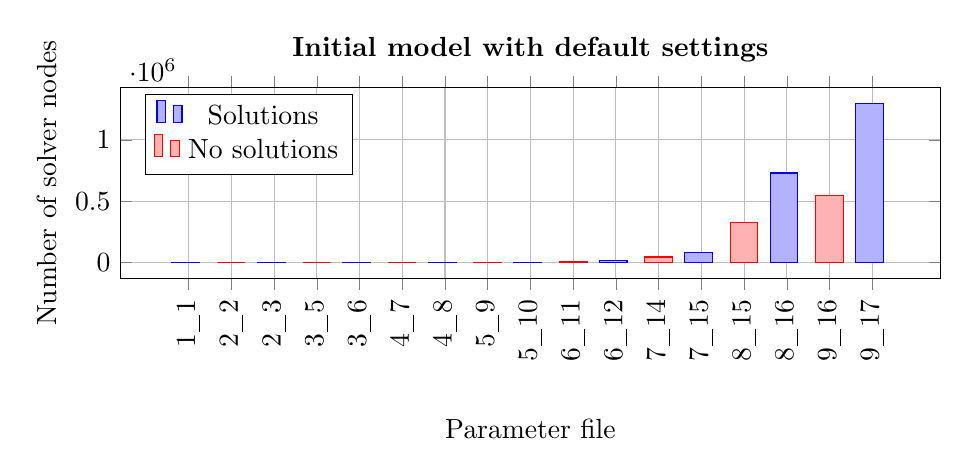
\begin{tikzpicture}
\begin{axis}[
	title={\textbf{Initial model with default settings}},
	ybar,
	bar width=1em,
	width=12cm,
	height=4cm,
	ylabel={Number of solver nodes},
	%ymode=log,
	xlabel={Parameter file},
	x label style={yshift=-0.5cm},
	xtick={1,2,3,4,5,6,7,8,9,10,11,12,13,14,15,16,17},
	xticklabels={1_1, 2_2, 2_3, 3_5, 3_6, 4_7, 4_8, 5_9, 5_10, 6_11, 6_12, 7_14, 7_15, 8_15, 8_16, 9_16, 9_17},
	x tick label style={rotate=90, anchor=east},
	ymajorgrids=true,
	xmajorgrids=true,
	legend pos=north west,
]

\addplot+[
xshift=0.5em, 
legend image post style={xshift=-0.5em}
] 
coordinates { (1,1) (3,1) (5,19) (7,18) (9,615) (11,14036) (13,82920) (15,730243) (17,1295303) };
\label{plot:solution-node}
\addlegendentry{Solutions}

\addplot+[
xshift=-0.6em,
legend image post style={xshift=0.5em}
] 
coordinates { (2,0) (4,0) (6,0) (8,267) (10,7052) (12,44769) (14,328143) (16,547184) };
\label{plot:nosolution-node}
\addlegendentry{No solutions}

\end{axis}
\end{tikzpicture}
\n
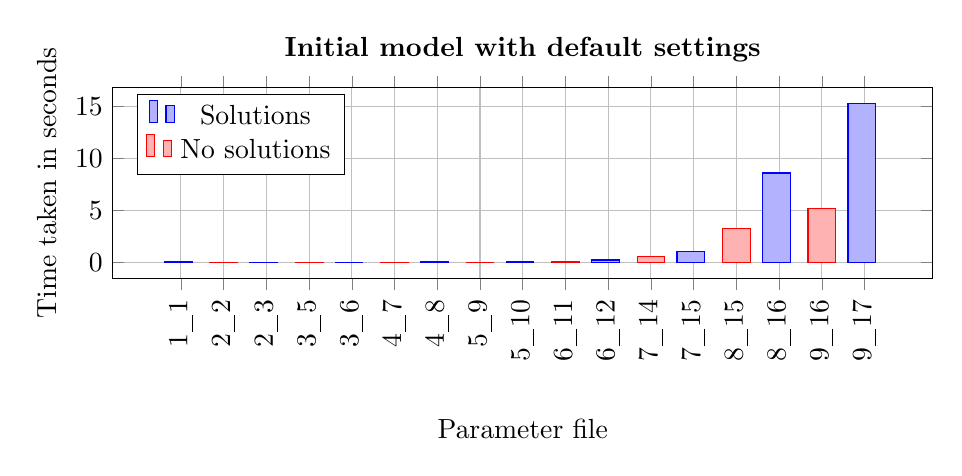
\begin{tikzpicture}
\begin{axis}[
	title={\textbf{Initial model with default settings}},
	ybar,
	bar width=1em,
	width=12cm,
	height=4cm,
	ylabel={Time taken in seconds},
	%ymode=log,
	xlabel={Parameter file},
	x label style={yshift=-0.5cm},
	xtick={1,2,3,4,5,6,7,8,9,10,11,12,13,14,15,16,17},
	xticklabels={1_1, 2_2, 2_3, 3_5, 3_6, 4_7, 4_8, 5_9, 5_10, 6_11, 6_12, 7_14, 7_15, 8_15, 8_16, 9_16, 9_17},
	x tick label style={rotate=90, anchor=east},
	ymajorgrids=true,
	xmajorgrids=true,
	legend pos=north west,
]

\addplot+[
xshift=0.5em, 
legend image post style={xshift=-0.5em}
] 
coordinates { (1,0.065969) (3,0.033876) (5,0.035081) (7,0.03787) (9,0.042356) (11,0.230148) (13,1.09208) (15,8.58716) (17,15.2453) };
\label{plot:solution-node}
\addlegendentry{Solutions}

\addplot+[
xshift=-0.6em,
legend image post style={xshift=0.5em}
] 
coordinates { (2,2.6e-05) (4,0.000738) (6,0.00137) (8,0.007254) (10,0.094615) (12,0.529334) (14,3.22285) (16,5.19558) };
\label{plot:nosolution-node}
\addlegendentry{No solutions}

\end{axis}
\end{tikzpicture}
\caption{Number of solver nodes and time taken on all given parameters for the initial model. The two different coloured bars represent parameters which either had a solution, or the solver found no solutions.}
\end{figure}
\noindent
At first glance, it appears that the instances with solutions always take more time and nodes than an instance of the same problem with no solution. This is not intuitive as logically having no solution means the solver must search through all nodes before stopping while having a solution means a solver can stop on the first solution found. However, it is unfair to make this comparison because the instance with solutions always contain one more step compared to their counterparts. We shall revisit this issue later by defining instances with multiple solutions and instances with more steps. 

\begin{figure}[H]
\centering
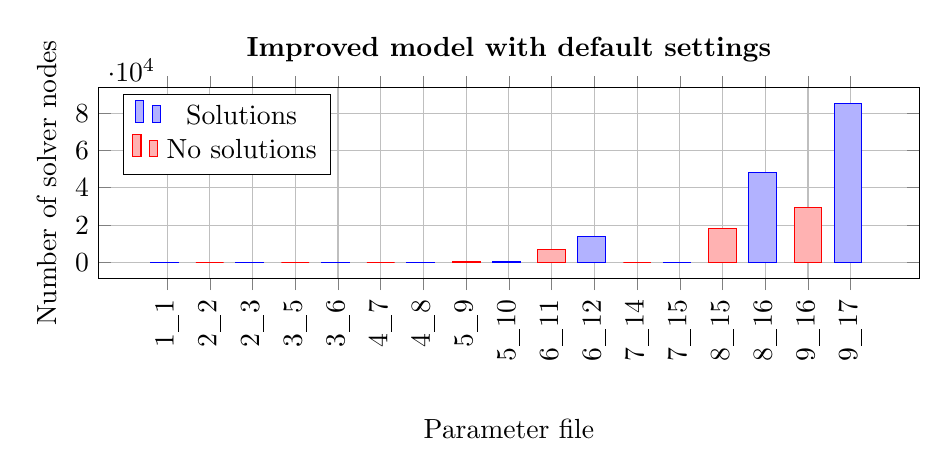
\begin{tikzpicture}
\begin{axis}[
	title={\textbf{Improved model with default settings}},
	ybar,
	bar width=1em,
	width=12cm,
	height=4cm,
	ylabel={Number of solver nodes},
	%ymode=log,
	xlabel={Parameter file},
	x label style={yshift=-0.5cm},
	xtick={1,2,3,4,5,6,7,8,9,10,11,12,13,14,15,16,17},
	xticklabels={1_1, 2_2, 2_3, 3_5, 3_6, 4_7, 4_8, 5_9, 5_10, 6_11, 6_12, 7_14, 7_15, 8_15, 8_16, 9_16, 9_17},
	x tick label style={rotate=90, anchor=east},
	ymajorgrids=true,
	xmajorgrids=true,
	legend pos=north west,
]

\addplot+[
xshift=0.5em, 
legend image post style={xshift=-0.5em}
] 
coordinates { (1,1) (3,1) (5,19) (7,1) (9,615) (11,13737) (13,1) (15,48055) (17,85000) };
\addlegendentry{Solutions}

\addplot+[
xshift=-0.6em,
legend image post style={xshift=0.5em}
] 
coordinates { (2,0) (4,0) (6,0) (8,267) (10,6786) (12,0) (14,18169) (16,29331) };
\addlegendentry{No solutions}
\end{axis}
\end{tikzpicture}
\n
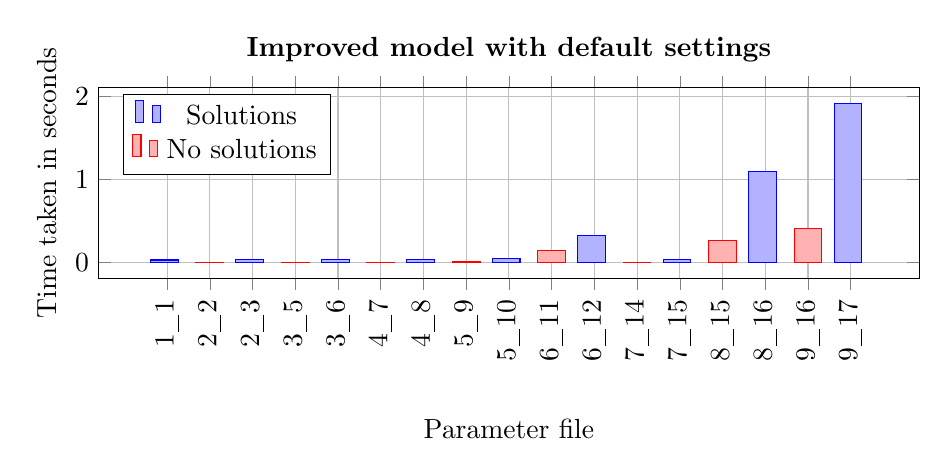
\begin{tikzpicture}
\begin{axis}[
	title={\textbf{Improved model with default settings}},
	ybar,
	bar width=1em,
	width=12cm,
	height=4cm,
	ylabel={Time taken in seconds},
	%ymode=log,
	xlabel={Parameter file},
	x label style={yshift=-0.5cm},
	xtick={1,2,3,4,5,6,7,8,9,10,11,12,13,14,15,16,17},
	xticklabels={1_1, 2_2, 2_3, 3_5, 3_6, 4_7, 4_8, 5_9, 5_10, 6_11, 6_12, 7_14, 7_15, 8_15, 8_16, 9_16, 9_17},
	x tick label style={rotate=90, anchor=east},
	ymajorgrids=true,
	xmajorgrids=true,
	legend pos=north west,
]

\addplot+[
xshift=0.5em, 
legend image post style={xshift=-0.5em}
] 
coordinates { (1,0.029641) (3,0.031378) (5,0.037638) (7,0.03456) (9,0.051029) (11,0.321407) (13,0.031937) (15,1.09181) (17,1.91063) };
\addlegendentry{Solutions}

\addplot+[
xshift=-0.6em,
legend image post style={xshift=0.5em}
] 
coordinates { (2,0.000611) (4,0.00091) (6,0.000311) (8,0.00986) (10,0.139993) (12,0.003395) (14,0.263946) (16,0.409637) };
\addlegendentry{No solutions}

\end{axis}
\end{tikzpicture}
\caption{Number of solver nodes and time taken on all given parameters for the improved model}
\end{figure}
\noindent
The improved model follows almost the same pattern as initial model, but the number of solver nodes and time taken is decreased significantly. For example the instance \texttt{9\_17} took over 15 seconds and 1 million solver nodes for the initial model while the improved model only took 2 seconds and 85000 nodes. This indicates the improved constraints help reduce the effort required by the solver by being more precise. Interestingly, problem 7 is easier for the improved model to solve and is an anomaly to the pattern of increasing time and number of nodes. 

\subsubsection{Optimisations}\label{sec:optimisation}
To find out more about Savile Row and our models, we can specify the level of optimisation. 
\begin{figure}[H]
\centering
\begin{minipage}{0.45\textwidth}
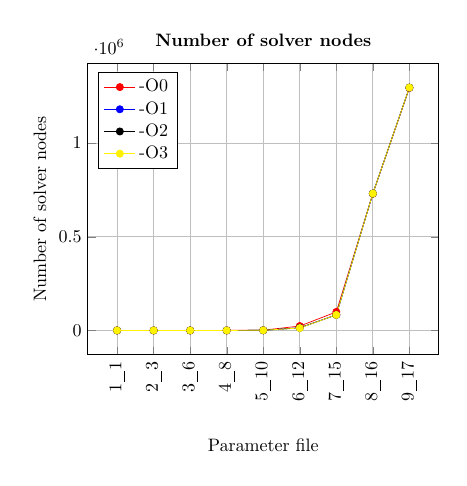
\begin{tikzpicture}[scale=0.65]
\begin{axis}[
	title={\textbf{Number of solver nodes}},
	ylabel={Number of solver nodes},
	%ymode=log,
	xlabel={Parameter file},
	x label style={yshift=-0.5cm},
	xtick={1,3,5,7,9,11,13,15,17},
	xticklabels={1_1, 2_3, 3_6, 4_8, 5_10, 6_12, 7_15, 8_16, 9_17},
	x tick label style={rotate=90, anchor=east},
	ymajorgrids=true,
	xmajorgrids=true,
	legend pos=north west,
	cycle list name=color list,
	]

\addplot+[mark=*] coordinates {
(1,1) (3,1) (5,21) (7,266) (9,1322) (11,23368) (13,98601) (15,729172) (17,1293411) };
\addlegendentry{-O0}

\addplot+[mark=*] coordinates {
(1,1) (3,1) (5,19) (7,18) (9,615) (11,14036) (13,82920) (15,730259) (17,1295335)};
\addlegendentry{-O1}

\addplot+[mark=*] coordinates {
(1,1) (3,1) (5,19) (7,18) (9,615) (11,14036) (13,82920) (15,730259) (17,1295335)};
\addlegendentry{-O2}

\addplot+[mark=*] coordinates {
(1,1) (3,1) (5,19) (7,18) (9,615) (11,12838) (13,82920) (15,730259) (17,1295335)};
\addlegendentry{-O3}
\end{axis}
\end{tikzpicture}
\end{minipage}
\hspace{0.4cm}
\begin{minipage}{0.45\textwidth}
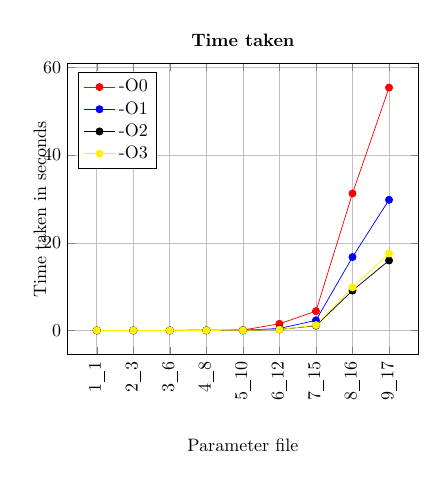
\begin{tikzpicture}[scale=0.65]
\begin{axis}[
	title={\textbf{Time taken}},
	ylabel={Time taken in seconds},
	y label style={yshift=-0.3cm},
	%ymode=log,
	xlabel={Parameter file},
	x label style={yshift=-0.5cm},
	xtick={1,3,5,7,9,11,13,15,17},
	xticklabels={1_1, 2_3, 3_6, 4_8, 5_10, 6_12, 7_15, 8_16, 9_17},
	x tick label style={rotate=90, anchor=east},
	ymajorgrids=true,
	xmajorgrids=true,
	legend pos=north west,
	cycle list name=color list,
	]

\addplot+[mark=*] coordinates {
(1,0.034987) (3,0.037164) (5,0.049465) (7,0.066688) (9,0.123698) (11,1.54227) (13,4.42801) (15,31.2728) (17,55.4183)
};
\addlegendentry{-O0}

\addplot+[mark=*] coordinates {
(1,0.03391) (3,0.033884) (5,0.041397) (7,0.055702) (9,0.066537) (11,0.476045) (13,2.33189) (15,16.768) (17,29.8262)};
\addlegendentry{-O1}

\addplot+[mark=*] coordinates {
(1,0.034406) (3,0.033279) (5,0.037437) (7,0.037128) (9,0.045367) (11,0.239904) (13,1.1221) (15,9.12738) (17,15.9849)};
\addlegendentry{-O2}

\addplot+[mark=*] coordinates {
(1,0.034467) (3,0.037342) (5,0.036098) (7,0.037964) (9,0.045614) (11,0.228288) (13,1.22769) (15,9.84382) (17,17.5615)};
\addlegendentry{-O3}

\end{axis}
\end{tikzpicture}
\end{minipage}
\caption{Comparing the effect of optimisation flags on the number of nodes and time taken on the initial model for parameter files with solutions. See appendix \ref{apdx:opt-flags} for full results.}
\end{figure}
\noindent
An interesting result from using different optimisation flags in is the effect it has on the performance of the model. Although it was shown earlier that the number of solver nodes and the time taken by the solver are very similar metrics for measuring the performance of the model, the optimisation flags have a much greater effect on the time taken compared to the number of nodes the solver has to search. With optimisations, the number of solver nodes only decreased by a small fraction. For many parameter files, this number did not change between the three levels of optimisation. However for the time taken by the solver, the time almost halved for most parameter files when comparing \texttt{-O0} and \texttt{-O1}. The time again decreased significantly for \texttt{-O2}, though there is little difference between \texttt{-O2} and \texttt{-O3}.
\n
This shows us that the optimisation does less to cull search nodes, but perhaps more to reduce processing time in generating the nodes or does more to be able to search through the nodes efficiently, especially as the problem sizes and complexity grows (size and complexity here refer to larger grids and more complicated grid setups like having ice blocks or multiple blocks to push). 
\n
That is not to say the optimisations have no effect at all on the solver nodes. Figure \ref{fig:optimisation-nodes} shows that for some parameter files, the optimisation does well enough to eliminate many solver nodes. For example in problems 4 and 7, the \texttt{-O1} optimisation is able to eliminate all but 1 solver node. From the difference shown between the initial model and improved model, it can be seen that the optimisations have a stronger effect on the better model for lowering the number of solver nodes. This shows it is important to have a well defined model as optimisations are not enough to overcome an inefficient model and are also more effective for good models. 
\begin{figure}[H]
\centering
\begin{minipage}{0.45\textwidth}
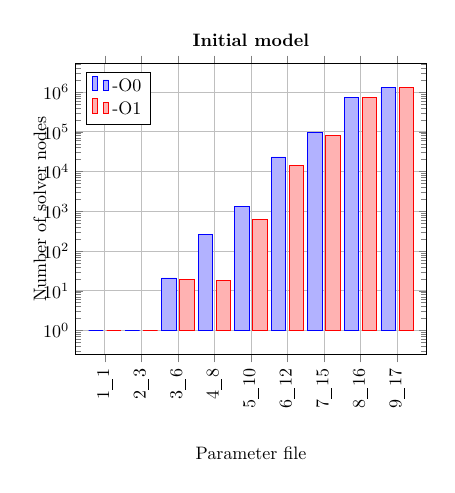
\begin{tikzpicture}[scale=0.65]
\begin{axis}[
	title={\textbf{Initial model}},
	ybar,
	bar width=0.8em,
	ylabel={Number of solver nodes},
	y label style={yshift=-0.3cm},
	ymode=log,
	xlabel={Parameter file},
	x label style={yshift=-0.5cm},
	xtick={1,3,5,7,9,11,13,15,17},
	xticklabels={1_1, 2_3, 3_6, 4_8, 5_10, 6_12, 7_15, 8_16, 9_17},
	x tick label style={rotate=90, anchor=east},
	ymajorgrids=true,
	xmajorgrids=true,
	legend pos=north west,
	]

\addplot coordinates {
(1,1) (3,1) (5,21) (7,266) (9,1322) (11,23368) (13,98601) (15,729172) (17,1293411)
};
\addlegendentry{-O0}

\addplot coordinates {
(1,1) (3,1) (5,19) (7,18) (9,615) (11,14036) (13,82920) (15,730259) (17,1295335)};
\addlegendentry{-O1}
\end{axis}
\end{tikzpicture}
\end{minipage}
\hspace{0.5cm}
\begin{minipage}{0.45\textwidth}
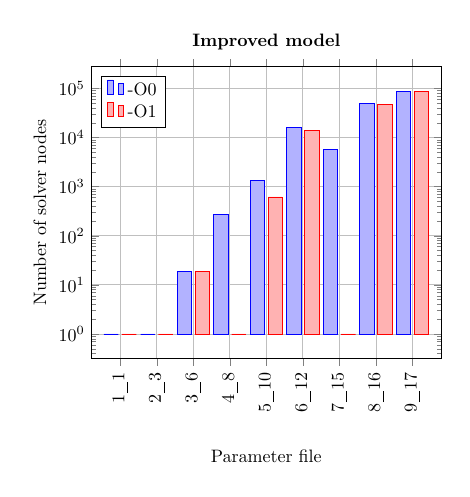
\begin{tikzpicture}[scale=0.65]
\begin{axis}[
	title={\textbf{Improved model}},
	ybar,
	bar width=0.8em,
	ylabel={Number of solver nodes},
	ymode=log,
	xlabel={Parameter file},
	x label style={yshift=-0.5cm},
	xtick={1,3,5,7,9,11,13,15,17},
	xticklabels={1_1, 2_3, 3_6, 4_8, 5_10, 6_12, 7_15, 8_16, 9_17},
	x tick label style={rotate=90, anchor=east},
	ymajorgrids=true,
	xmajorgrids=true,
	legend pos=north west,
	]

\addplot coordinates {
(1,1) (3,1) (5,19) (7,266) (9,1313) (11,16198) (13,5755) (15,49723) (17,88077)
};
\addlegendentry{-O0}

\addplot coordinates {
(1,1) (3,1) (5,19) (7,1) (9,615) (11,13737) (13,1) (15,48055) (17,85000)};
\addlegendentry{-O1}
\end{axis}
\end{tikzpicture}
\end{minipage}
\caption{Effect of optimisation flags on number of solver nodes for parameter files with solutions.}
\label{fig:optimisation-nodes}
\end{figure}

\subsubsection{Heuristics}
Another option to look at is the heuristics that Essence Prime provides. As these are heuristics that must be specified in the model (in \texttt{Bombastic.eprime}), we are interested to see how they may affect the number of solver nodes searched by the model. Many of the problem instances follow a similar pattern for how they are affected by different heuristics. We shall focus our attention on the \texttt{9\_17} problem instance as it is the most difficult problem - takes the longest time and most solver nodes - and allows us to find patterns without having too complex a graph.
\n
From figure \ref{fig:heuristics}, the most interesting heuristics to take note of are \texttt{sdf} and \texttt{srf}. When using the \texttt{sdf} heuristic, we can see there is a large difference for its effect on the initial model and improved model. With optimisation flags, the heuristic causes the model to perform \textit{worse} than without any optimisation for the initial model, but it performs well for the improved model only with optimisations on. It is impossible to say without knowing what the heuristics do how the models are actually affected, but the more concise constraints of the improved model are likely part of the cause. 
\n
In the case of \texttt{srf}, we again have some very interesting results. The effect of using \texttt{srf} combined with optimisations seem to have almost an opposite effect on the two models. \texttt{O1} optimisation performs worse than \texttt{O0} and \texttt{O2} and \texttt{O3} perform the best for the initial model. This directly contrasts the results for the improved model, where \texttt{O1} performs the best, \texttt{O0} the worst, but turning on higher optimisations (\texttt{O2} and \texttt{O3}) increases the number of solver nodes compared to \texttt{O1}. There may be some work that the heuristic does that additional optimisations do not take advantage of or their combination conflicts with each other. Of course, even though \texttt{srt} performs better on higher optimisations for the initial model, the number of nodes is still greater. 

\begin{figure}[H]
\centering
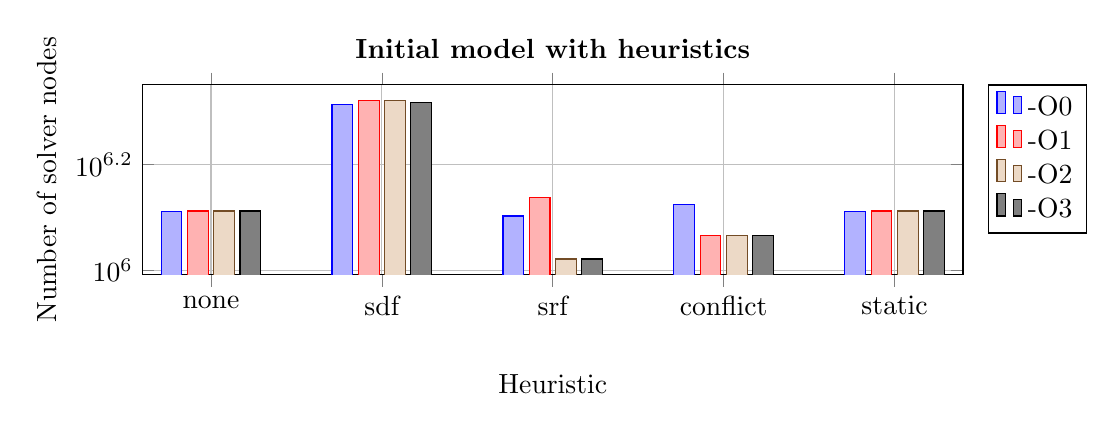
\begin{tikzpicture}
\begin{axis}[
	title={\textbf{Initial model with heuristics}},
	ybar,
	bar width=0.75em,
	width=12cm,
	height=4cm,
	ylabel={Number of solver nodes},
	ymode=log,
	xlabel={Heuristic},
	x label style={yshift=-0.5cm},
	symbolic x coords={none, sdf, srf, conflict, static},
	xtick=data,
	ymajorgrids=true,
	xmajorgrids=true,
	legend pos=outer north east,
]

\addplot
coordinates {
(none,1293411) (sdf,2057773) (conflict,1331953) (static,1293411) (srf,1267730)
};
\addlegendentry{-O0}

\addplot
coordinates {
(none,1295335) (sdf,2096419) (conflict,1163274) (static,1295335) (srf,1373057)
};
\addlegendentry{-O1}

\addplot
coordinates {
(none,1295335) (sdf,2093815) (conflict,1163274) (static,1295335) (srf,1051399)
};
\addlegendentry{-O2}

\addplot
coordinates {
(none,1295335) (sdf,2079703) (conflict,1163274) (static,1295335) (srf,1051399)
};
\addlegendentry{-O3}

\end{axis}
\end{tikzpicture}
\n
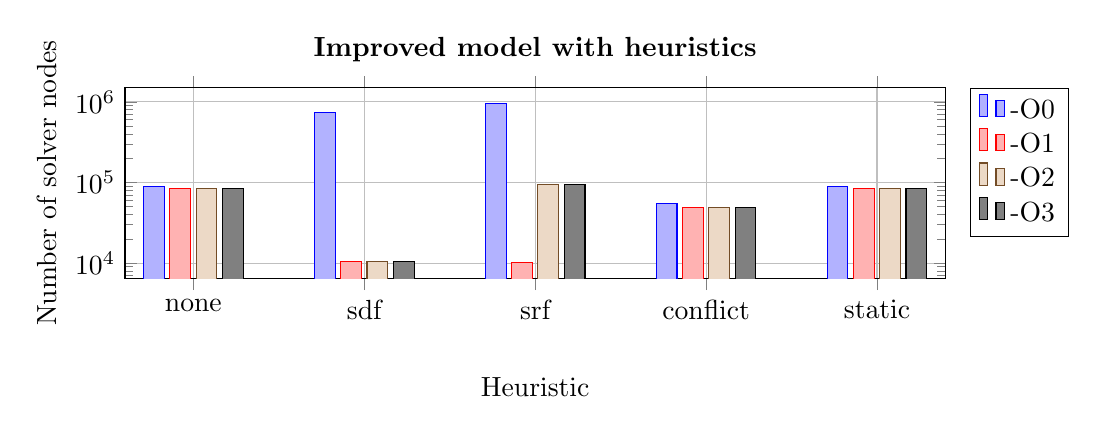
\begin{tikzpicture}
\begin{axis}[
	title={\textbf{Improved model with heuristics}},
	ybar,
	bar width=0.75em,
	width=12cm,
	height=4cm,
	ylabel={Number of solver nodes},
	ymode=log,
	xlabel={Heuristic},
	x label style={yshift=-0.5cm},
	symbolic x coords={none, sdf, srf, conflict, static},
	xtick=data,
	ymajorgrids=true,
	xmajorgrids=true,
	legend pos=outer north east,
]

\addplot
coordinates {
(none,88077) (sdf,745796) (conflict,54783) (static,88077) (srf,946285)
};
\addlegendentry{-O0}

\addplot
coordinates {
(none,85000) (sdf,10379) (conflict,48609) (static,85000) (srf,10185)
};
\addlegendentry{-O1}

\addplot
coordinates {
(none,85000) (sdf,10379) (conflict,48609) (static,85000) (srf,94843)
};
\addlegendentry{-O2}

\addplot
coordinates {
(none,85000) (sdf,10379) (conflict,48609) (static,85000) (srf,94843)
};
\addlegendentry{-O3}

\end{axis}
\end{tikzpicture}
\caption{Effect of different heuristics on problem instance \texttt{9\_17}}
\label{fig:heuristics}
\end{figure}

\noindent
It is important to note that these results and patterns are not unique to the \texttt{9\_17} instance and recurs in many of the given instances. Furthermore, it should also be noted that in the case of \texttt{sdf} and \texttt{srf}, using the heuristics without optimisations performs worse than not using the heuristics at all. This suggests some kind of relationship between how the heuristics and optimisations complement or contrast each other. Perhaps the heuristics create a lot of equivalent or symmetrical nodes that optimisations can easily simplify, but over-complicates the search if not simplified.

\subsection{Custom instances}
To look into more detail at how the effort required of the models are affected, some of the given instances have been modified and tested against the improved model. This allows us to more finely test what affects the efficiency of the model and isolate specific variables to change and test.


\subsubsection{Increasing number of steps}
First, a simple thing we can change is the number of steps for problems we looked at earlier. This gives us a comparison against earlier results. The number of steps is increased and not decreased as decreasing the number of steps will only lead to having no solution due to the nature of the game. We test this for both problems with solutions after increasing the number of steps, and problems with no solutions after. Examples of the latter would be grids that contain ice such that the avatar cannot move after pushing all blocks into goals, thereby causing no solution to be found. We use default settings here only on the improved model as we want to focus our attention on the effect of the parameter files and not on other options explored earlier. 

\begin{figure}[H]
\centering

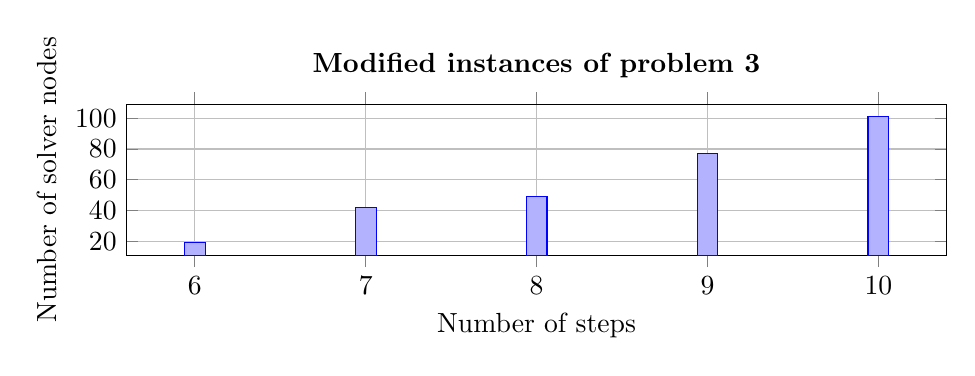
\begin{tikzpicture}
\begin{axis}[
	title={\textbf{Modified instances of problem 3}},
	ybar,
	bar width=0.75em,
	width=12cm,
	height=3.5cm,
	ylabel={Number of solver nodes},
	%ymode=log,
	xlabel={Number of steps},
	%x label style={yshift=-0.5cm},
	symbolic x coords={6,7,8,9,10},
	xtick=data,
	%x tick label style={rotate=90, anchor=east},
	ymajorgrids=true,
	xmajorgrids=true,
	legend pos=outer north east,
]
\addplot
coordinates {
(6,19) (7,42) (8,49) (9,77) (10,101) 
};
\end{axis}
\end{tikzpicture}
\n
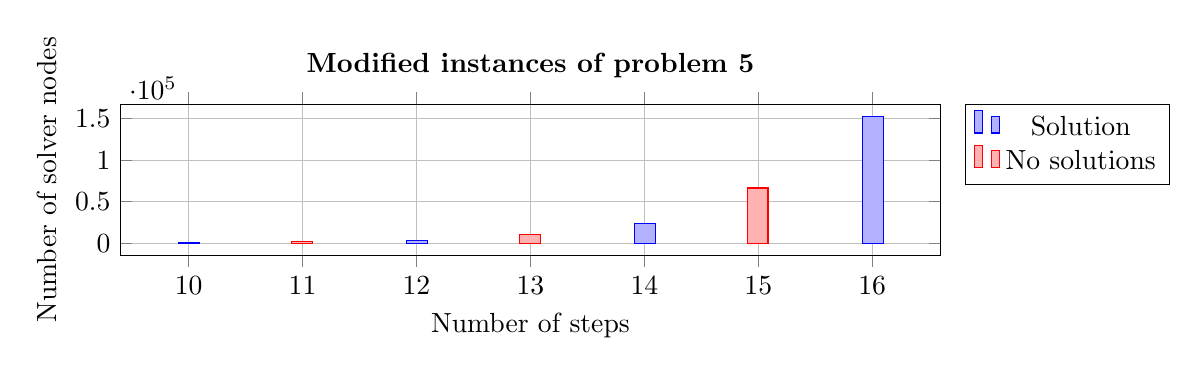
\begin{tikzpicture}
\begin{axis}[
	title={\textbf{Modified instances of problem 5}},
	ybar,
	bar width=0.75em,
	width=12cm,
	height=3.5cm,
	ylabel={Number of solver nodes},
	%ymode=log,
	xlabel={Number of steps},
	%x label style={yshift=-0.5cm},
	symbolic x coords={10,11,12,13,14,15,16},
	%x tick label style={rotate=90, anchor=east},
	ymajorgrids=true,
	xmajorgrids=true,
	legend pos=outer north east,
]

\addplot+[
	xshift=0.5em,
	legend image post style={xshift=-0.5em}	
]
coordinates {
(10,615) (12,3617) (14,23315) (16,152245)
};
\addlegendentry{Solution}

\addplot+[
	xshift=-0.5em,
	legend image post style={xshift=0.5em}	
]
coordinates {
(11,1611) (13,10278) (15,66518)
};
\addlegendentry{No solutions}

\end{axis}
\end{tikzpicture}

\caption{Number of nodes on the same problems but with varying number of steps required. Note that for problem 5, the number of steps determines whether there is a solution or not as the avatar can move back and forth along his initial position with two extra steps, but not with just one extra step. For problem 3, all instances have solutions as the avatar can move freely after pushing all blocks into the goal.}
\end{figure}
\noindent
It is interesting to see how the number of solver nodes increases with the number of steps even though there is still just one or no solution. This suggests that the number of steps is an independent factor in regards to the difficulty of a problem instance. It also doesn't seem to matter whether the increased steps led to a solution or not as the number of nodes increases regardless. Sequences of movement after the blocks are pushed into the goals for problem 3 should not increase the number of solver nodes, since any sequence of movement after the blocks are pushed is a valid solution and the solver would stop. This means the nodes must come from large numbers of backtracking combinations before the block is pushed into the goal that are tried because having more steps increased the number of combinations. The increased work from a larger grid may also dwarf the work difference between problems with and without a solution. It is difficult to test the same problem instance both with and without a solution since the problem would be a different instance by definition, but we can certainly say the number of steps is a large factor in the difficulty of the Bombastic problem. 


\subsubsection{Increasing cube problems}
Something that we want to test is how a problem with multiple solutions would affect our model, especially when the \texttt{-all-solutions} flag is passed into Savile Row. A custom instance that was created and tested for this purpose was an $n \times n$ cube where the avatar always started at the top left, the goal is always at the bottom right and the one single block is always on the cell directly top left of the goal. The $n \times n$ here is the size of the live cells in the problem grid, not taking into account the ring of dead cells. 

\begin{figure}[H]
\centering
\begin{tabular}{ | c | c | c | c | c | }
\hline
0 & 0 & 0 & 0 & 0 \\ \hline
0 & \textbf{P} & 2 & 2 & 0 \\ \hline
0 & 2 & \textbf{B} & 2 & 0 \\ \hline
0 & 2 & 2 & \textbf{G} & 0 \\ \hline
0 & 0 & 0 & 0 & 0 \\ \hline
\end{tabular}
\hspace{1cm}
\begin{tabular}{ | c | c | c | c | c | c | c | c | }
\hline
0 & 0 & 0 & 0 & 0 & 0 & 0 & 0 \\ \hline
0 & \textbf{P} & 2 & 2 & 2 & 2 & 2 & 0 \\ \hline
0 & 2 & 2 & 2 & 2 & 2 & 2 & 0 \\ \hline
0 & 2 & 2 & 2 & 2 & 2 & 2 & 0 \\ \hline
0 & 2 & 2 & 2 & 2 & 2 & 2 & 0 \\ \hline
0 & 2 & 2 & 2 & 2 & \textbf{B} & 2 & 0 \\ \hline
0 & 2 & 2 & 2 & 2 & 2 & \textbf{G} & 0 \\ \hline
0 & 0 & 0 & 0 & 0 & 0 & 0 & 0 \\ \hline
\end{tabular}
\caption{Examples of a $3 \times 3$ and $6 \times 6$ cube problem instance on the left and right respectively.}
\end{figure}
\noindent
Cube problem sizes from $3 \times 3$ to $9 \times 9$ were created and run with the improved model. This problem is used to test two different aspects of the model and solver. First is how the size of the grid affects the time and number of nodes to find a solution. This is different from the initial testing with the given parameter files as there is no increased complexity in the problem instance from elements such as ice blocks and multiple blocks. Only the size of the grid changes between cube problem instances. Secondly we can test the effect of multiple solutions to confirm the solver takes more time and nodes as there are more solutions to a problem instance.

\begin{figure}[H]
\centering
\begin{minipage}{0.45\textwidth}
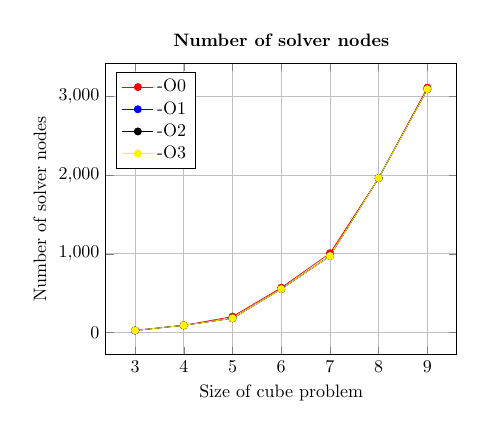
\begin{tikzpicture}[scale=0.65]
\begin{axis}[
	title={\textbf{Number of solver nodes}},
	%ybar,
	ylabel={Number of solver nodes},
	%ymode=log,
	xlabel={Size of cube problem},
	%x label style={yshift=-0.5cm},
	xtick={1,2,3,4,5,6,7},
	xticklabels={3,4,5,6,7,8,9},
	ymajorgrids=true,
	xmajorgrids=true,
	legend pos=north west,
	cycle list name=color list,
	]

\addplot+[mark=*] coordinates {
(1,26) (2,91) (3,202) (4,569) (5,1007) (6,1961) (7,3111) };
\addlegendentry{-O0}

\addplot+[mark=*] coordinates {
(1,26) (2,91) (3,180) (4,552) (5,971) (6,1961) (7,3091)};
\addlegendentry{-O1}

\addplot+[mark=*] coordinates {
(1,26) (2,91) (3,180) (4,552) (5,971) (6,1961) (7,3091)};
\addlegendentry{-O2}

\addplot+[mark=*] coordinates {
(1,26) (2,91) (3,180) (4,552) (5,971) (6,1961) (7,3091)};
\addlegendentry{-O3}

\end{axis}

\end{tikzpicture}
\end{minipage}
%
\begin{minipage}{0.45\textwidth}
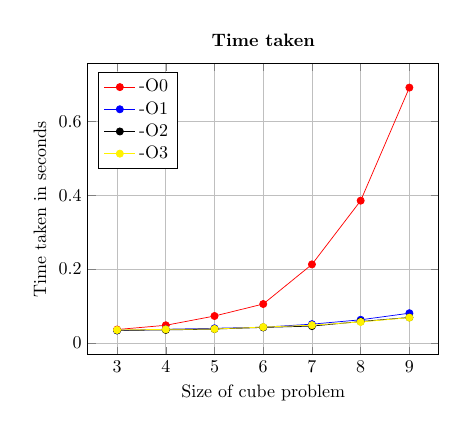
\begin{tikzpicture}[scale=0.65]
\begin{axis}[
	title={\textbf{Time taken}},
	%ybar,
	ylabel={Time taken in seconds},
	%ymode=log,
	xlabel={Size of cube problem},
	%x label style={yshift=-0.5cm},
	xtick={1,2,3,4,5,6,7},
	xticklabels={3,4,5,6,7,8,9},
	ymajorgrids=true,
	xmajorgrids=true,
	legend pos=north west,
	cycle list name=color list,
	]

\addplot+[mark=*] coordinates {
(1,0.036699) (2,0.048209) (3,0.073289) (4,0.105752) (5,0.213041) (6,0.385509) (7,0.691582) 
};
\addlegendentry{-O0}

\addplot+[mark=*] coordinates {
(1,0.034287) (2,0.037479) (3,0.040116) (4,0.043055) (5,0.051263) (6,0.063065) (7,0.080922) };
\addlegendentry{-O1}

\addplot+[mark=*] coordinates {
(1,0.034397) (2,0.035583) (3,0.03793) (4,0.042398) (5,0.045988) (6,0.058425) (7,0.06942)};
\addlegendentry{-O2}

\addplot+[mark=*] coordinates {
(1,0.035515) (2,0.037177) (3,0.03824) (4,0.04338) (5,0.048467) (6,0.057125) (7,0.069001)};
\addlegendentry{-O3}

\end{axis}
\end{tikzpicture}
\end{minipage}
\caption{Results of running all cube problems without the \texttt{-all-solutions} flag.}
\label{fig:cube-one}
\end{figure}
\noindent
We can see that as the size of the grid increases, the number of solver nodes searched increases exponentially. This makes sense as the size of the grid and number of steps has increased, there is a larger search space with more possible moves to search through. What is interesting is that the time taken is significantly improved by the optimisations while the number of solver nodes is not. This is similar to the pattern observed in section \ref{sec:optimisation} but to a greater effect. 

\begin{figure}[H]
\centering
\begin{minipage}{0.45\textwidth}
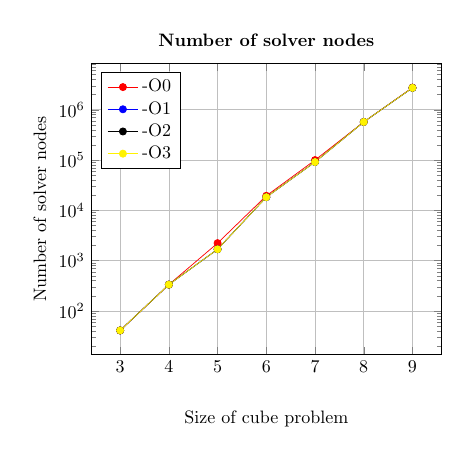
\begin{tikzpicture}[scale=0.65]
\begin{axis}[
	title={\textbf{Number of solver nodes}},
	%ybar,
	ylabel={Number of solver nodes},
	ymode=log,
	xlabel={Size of cube problem},
	x label style={yshift=-0.5cm},
	xtick={1,2,3,4,5,6,7},
	xticklabels={3,4,5,6,7,8,9},
	ymajorgrids=true,
	xmajorgrids=true,
	legend pos=north west,
	cycle list name=color list,
	]

\addplot+[mark=*] coordinates {
(1,41) (2,334) (3,2231) (4,19480) (5,99842) (6,571479) (7,2756393)};
\addlegendentry{-O0}

\addplot+[mark=*] coordinates {
(1,41) (2,334) (3,1685) (4,18290) (5,91490) (6,571479) (7,2721358)};
\addlegendentry{-O1}

\addplot+[mark=*] coordinates {
(1,41) (2,334) (3,1685) (4,18290) (5,91490) (6,571479) (7,2721358)};
\addlegendentry{-O2}

\addplot+[mark=*] coordinates {
(1,41) (2,334) (3,1685) (4,18290) (5,91490) (6,571479) (7,2721358)};
\addlegendentry{-O3}

\end{axis}

\end{tikzpicture}
\end{minipage}
%
\begin{minipage}{0.45\textwidth}
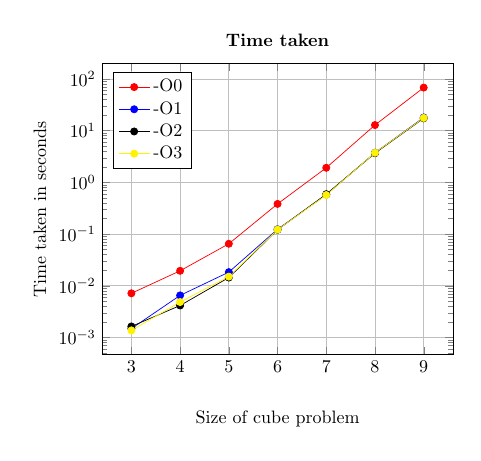
\begin{tikzpicture}[scale=0.65]
\begin{axis}[
	title={\textbf{Time taken}},
	%ybar,
	ylabel={Time taken in seconds},
	ymode=log,
	xlabel={Size of cube problem},
	x label style={yshift=-0.5cm},
	xtick={1,2,3,4,5,6,7},
	xticklabels={3,4,5,6,7,8,9},
	ymajorgrids=true,
	xmajorgrids=true,
	legend pos=north west,
	cycle list name=color list,
	]

\addplot+[mark=*] coordinates {
(1,0.007149) (2,0.019477) (3,0.064929) (4,0.383109) (5,1.91445) (6,12.8314) (7,68.0679)
};
\addlegendentry{-O0}

\addplot+[mark=*] coordinates {
(1,0.001486) (2,0.006518) (3,0.018368) (4,0.123967) (5,0.576449) (6,3.74547) (7,17.9922) };
\addlegendentry{-O1}

\addplot+[mark=*] coordinates {
(1,0.001634) (2,0.004154) (3,0.014428) (4,0.12099) (5,0.59102) (6,3.66499) (7,17.3433)};
\addlegendentry{-O2}

\addplot+[mark=*] coordinates {
(1,0.001369) (2,0.004841) (3,0.015021) (4,0.122008) (5,0.569325) (6,3.74015) (7,17.6333)};
\addlegendentry{-O3}

\end{axis}
\end{tikzpicture}
\end{minipage}
\caption{Results of running all cube problems finding all solutions. The y-axis is plot as a log axis to more clearly see the relation of the data.}
\label{fig:cube-all}
\end{figure}

\begin{figure}[H]
\centering
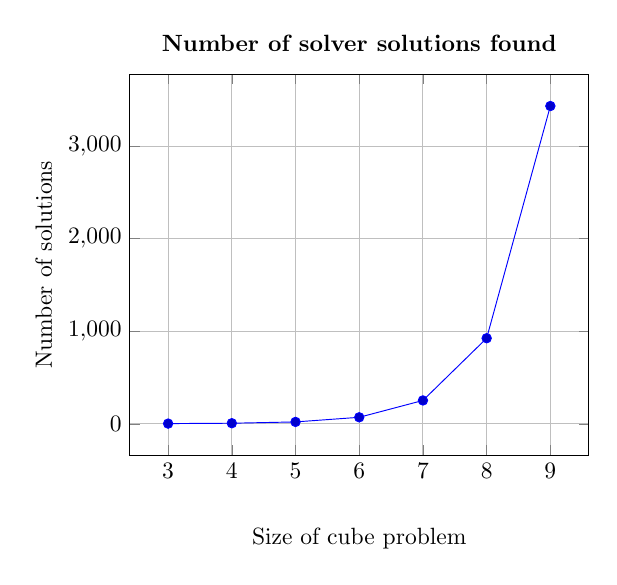
\begin{tikzpicture}[scale=0.85]
\begin{axis}[
	title={\textbf{Number of solver solutions found}},
	%ybar,
	ylabel={Number of solutions},
	%ymode=log,
	xlabel={Size of cube problem},
	x label style={yshift=-0.5cm},
	xtick={1,2,3,4,5,6,7},
	xticklabels={3,4,5,6,7,8,9},
	ymajorgrids=true,
	xmajorgrids=true,
	%legend pos=north west,
	%cycle list name=color list,
	]

\addplot+[mark=*] coordinates {
(1,2) (2,6) (3,20) (4,70) (5,252) (6,924) (7,3432)
};

\end{axis}
\end{tikzpicture}
\caption{Number of solutions found for each cube problem instance.}
\end{figure}
\noindent
Another good result we get is time and nodes searched to find all solutions is much more than just finding one solution. Though this should be obvious, it is a good result to show empirically, showing that the constraint solver will stop at the first solution found without any further searching by default.
\n
Again the same pattern of improving time with optimisations without improving the number of nodes applies when finding all solutions as well. The log graph of figure \ref{fig:cube-all} quite clearly shows no optimisations is worse for every sized cube problem instance. However, it is difficult to determine if this pattern is due solely to the increasing complexity from the size of the grid, as the number of steps had to be increased as well and it is already shown that the number of steps is an important factor where more steps requires more effort to solve.

\subsubsection{Cube with ice}
To determine whether the number of steps is the sole factor determining the effort required, we can change our cube problems to contain ice cells instead of normal cells. The number of steps stays constant for each cube problem, but all normal cells are replaced with ice cells. This does not affect the solution as all solutions with the given number of steps do not require walking back over any previously visited cell. In other words, it is valid to change all cells to ice without losing any solutions.
\begin{figure}[H]
\centering
\begin{minipage}{0.45\textwidth}
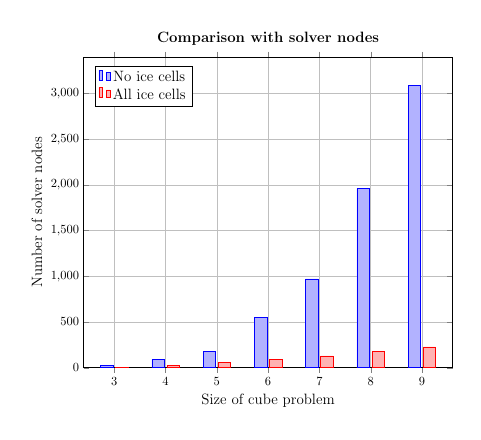
\begin{tikzpicture}[scale=0.45]
\begin{axis}[
	title={{\large \textbf{Comparison with solver nodes}}},
	ybar,
	bar width=1em,
	width=12cm,
	ylabel={{\large Number of solver nodes}},
	ymin=0,
	%ymode=log,
	xlabel={{\large Size of cube problem}},
	xtick={1,2,3,4,5,6,7},
	xticklabels={3,4,5,6,7,8,9},
	ymajorgrids=true,
	xmajorgrids=true,
	legend pos=north west,
	%cycle list name=color list,
	]

\addplot
coordinates {
(1,26) (2,91) (3,180) (4,552) (5,971) (6,1961) (7,3091)
};
\addlegendentry{{\large No ice cells}}

\addplot
coordinates {
(1,4) (2,28) (3,56) (4,90) (5,130) (6,176) (7,228)
};
\addlegendentry{{\large All ice cells}}

\end{axis}

\end{tikzpicture}
\end{minipage}
\hspace{0.5cm}
\begin{minipage}{0.45\textwidth}
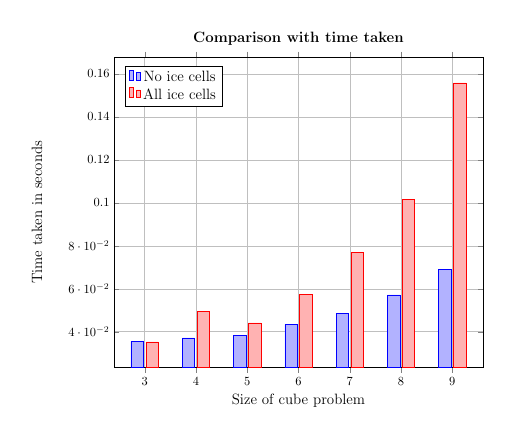
\begin{tikzpicture}[scale=0.45]
\begin{axis}[
	title={{\large \textbf{Comparison with time taken}}},
	ybar,
	bar width=1em,
	width=12cm,
	ylabel={{\large Time taken in seconds}},
	y label style={yshift=0.5cm},
	%ymode=log,
	xlabel={{\large Size of cube problem}},
	xtick={1,2,3,4,5,6,7},
	xticklabels={3,4,5,6,7,8,9},
	ymajorgrids=true,
	xmajorgrids=true,
	legend pos=north west,
	%cycle list name=color list,
	]

\addplot
coordinates {
(1,0.035515) (2,0.037177) (3,0.03824) (4,0.04338) (5,0.048467) (6,0.057125) (7,0.069001)
};
\addlegendentry{{\large No ice cells}}

\addplot
coordinates {
(1,0.035332) (2,0.049489) (3,0.044164) (4,0.057221) (5,0.07685) (6,0.101592) (7,0.155829)
};
\addlegendentry{{\large All ice cells}}

\end{axis}

\end{tikzpicture}
\end{minipage}
\caption{Comparison of the same cube problems with same steps but cells are either all normal or all ice.}
\label{fig:cube-ice}
\end{figure}
\noindent
Having the problem instances change to contain all ice cells dramatically decreases the number of solver nodes searched. The rest of the instance stays exactly the same, including the number of steps. This is interesting as it shows the ice creates less nodes to search through as it prevents any nodes with backtracking because it is not allowed to walk back from the ice. However, the time taken tells an opposite story. The problem instances with ice take \textit{more} time to solve even though there are many less nodes being searched. This shows the effort by the solver isn't just on searching through the nodes to find a solution, but also includes processing time to go through the constraints to get the nodes in the first place. Having all ice cells complicates the instance in that every move causes changes to the grid and therefore required more time. 
\n
From this, we can also say that the number of steps is not the only factor. The complexity of the instance changes the effort taken by the solver and model. A more complicated problem contains less search because it is more constrained by the model, but still takes time and effort as more constraints have to be processed. More steps does seem to be a large contributing factor, as figure \ref{fig:cube-ice} still shows a larger grid - which requires more steps to solve - takes more work, but there are other factors like the ice cells which can change the efficiency in which the model can find solutions.


\section{Conclusion}
In conclusion, two models with different constraints were developed and tested against various Bombastic problem instances. The second model attempted to improve on the first by simplifying complicated constraints to be more precise. The differences between the models are shown by their performance on the given problem instances. Additionally, the solver options of Savile Row such as optimisation flags and heuristics were also explored to see their effect on the two models. Finally, custom instances were created to isolate and test how specific elements increased the difficulty of the Bombastic problem and affected the performance of our constraints model.
\n
The optimisation flags and heuristics both had strong effects on the model, able to eliminate solver nodes and decrease the time taken by the model. The two seem to be able to work in tandem, producing good results if both are used. Nevertheless, using heuristics blindly without understanding how they work can have a negative impact on performance, as some combinations of heuristics and optimisations can lead to decreased performance. 
\n
Furthermore, it was found that the number of steps had a large impact on the effort required to solve the problem, as it led to more solver nodes and more time taken, even if the rest of the problem instance stays the same. It was also shown that there are other factors such as complexity of the instance that contribute to different efforts required to solve the problem.

\begin{appendices}
\counterwithin{figure}{section}
\section{Results of optimisation flags}\label{apdx:opt-flags}

\begin{figure}[H]
\centering
\begin{minipage}{0.45\textwidth}
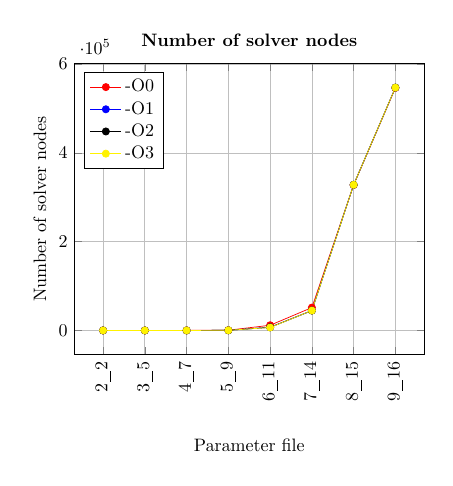
\begin{tikzpicture}[scale=0.65]
\begin{axis}[
	title={\textbf{Number of solver nodes}},
	ylabel={Number of solver nodes},
	%ymode=log,
	xlabel={Parameter file},
	x label style={yshift=-0.5cm},
	xtick={2,4,6,8,10,12,14,16},
	xticklabels={2_2,3_5,4_7,5_9,6_11,7_14,8_15,9_16},
	x tick label style={rotate=90, anchor=east},
	ymajorgrids=true,
	xmajorgrids=true,
	legend pos=north west,
	cycle list name=color list,
	]

\addplot+[mark=*] coordinates {
(2,0) (4,0) (6,113) (8,512) (10,11671) (12,51492) (14,327718) (16,546476) };
\addlegendentry{-O0}

\addplot+[mark=*] coordinates {
(2,0) (4,0) (6,0) (8,267) (10,7052) (12,44769) (14,328143) (16,547184)};
\addlegendentry{-O1}

\addplot+[mark=*] coordinates {
(2,0) (4,0) (6,0) (8,267) (10,7052) (12,44769) (14,328143) (16,547184)};
\addlegendentry{-O2}

\addplot+[mark=*] coordinates {
(2,0) (4,0) (6,0) (8,267) (10,6622) (12,44769) (14,328143) (16,547184) };
\addlegendentry{-O3}

\end{axis}

\end{tikzpicture}
\end{minipage}
%
\begin{minipage}{0.45\textwidth}
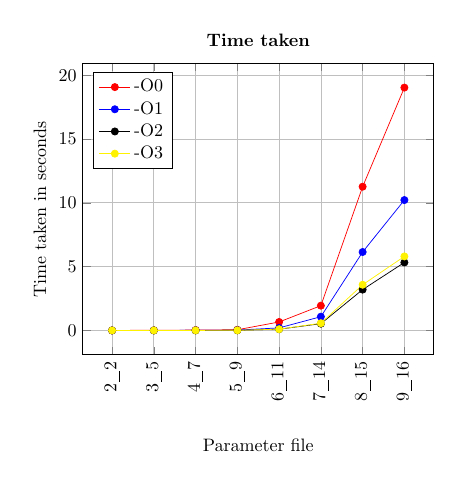
\begin{tikzpicture}[scale=0.65]
\begin{axis}[
	title={\textbf{Time taken}},
	ylabel={Time taken in seconds},
	%ymode=log,
	xlabel={Parameter file},
	x label style={yshift=-0.5cm},
	xtick={2,4,6,8,10,12,14,16},
	xticklabels={2_2,3_5,4_7,5_9,6_11,7_14,8_15,9_16},
	x tick label style={rotate=90, anchor=east},
	ymajorgrids=true,
	xmajorgrids=true,
	legend pos=north west,
	cycle list name=color list,
	]

\addplot+[mark=*] coordinates {
(2,0.002527) (4,0.008836) (6,0.030193) (8,0.052777) (10,0.662101) (12,1.94038) (14,11.2637) (16,19.0305)};
\addlegendentry{-O0}

\addplot+[mark=*] coordinates {
(2,0.000509) (4,0.002246) (6,0.007113) (8,0.02607) (10,0.199171) (12,1.07673) (14,6.14513) (16,10.2163)};
\addlegendentry{-O1}

\addplot+[mark=*] coordinates {
(2,0.000139) (4,0.000923) (6,0.001386) (8,0.00733) (10,0.095159) (12,0.529529) (14,3.19886) (16,5.32569)};
\addlegendentry{-O2}

\addplot+[mark=*] coordinates {
(2,1e-06) (4,0.000428) (6,0.001355) (8,0.008099) (10,0.097074) (12,0.565429) (14,3.57982) (16,5.7996)};
\addlegendentry{-O3}

\end{axis}
\end{tikzpicture}
\end{minipage}
\caption{Optimisations with initial model on problem files \textit{without} solutions}
\end{figure}

\vspace{0.5cm}

\begin{figure}[H]
\centering
\begin{minipage}{0.45\textwidth}
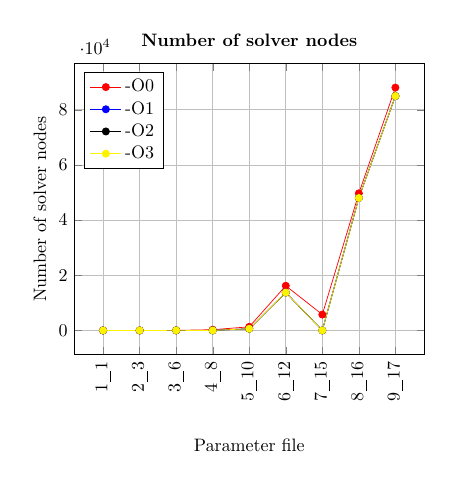
\begin{tikzpicture}[scale=0.65]
\begin{axis}[
	title={\textbf{Number of solver nodes}},
	ylabel={Number of solver nodes},
	%ymode=log,
	xlabel={Parameter file},
	x label style={yshift=-0.5cm},
	xtick={1,3,5,7,9,11,13,15,17},
	xticklabels={1_1, 2_3, 3_6, 4_8, 5_10, 6_12, 7_15, 8_16, 9_17},
	x tick label style={rotate=90, anchor=east},
	ymajorgrids=true,
	xmajorgrids=true,
	legend pos=north west,
	cycle list name=color list,
	]

\addplot+[mark=*] coordinates {
(1,1) (3,1) (5,19) (7,266) (9,1313) (11,16198) (13,5755) (15,49723) (17,88077) };
\addlegendentry{-O0}

\addplot+[mark=*] coordinates {
(1,1) (3,1) (5,19) (7,1) (9,615) (11,13737) (13,1) (15,48055) (17,85000)};
\addlegendentry{-O1}

\addplot+[mark=*] coordinates {
(1,1) (3,1) (5,19) (7,1) (9,615) (11,13737) (13,1) (15,48055) (17,85000)};
\addlegendentry{-O2}

\addplot+[mark=*] coordinates {
(1,1) (3,1) (5,19) (7,1) (9,615) (11,13737) (13,1) (15,48055) (17,85000) };
\addlegendentry{-O3}

\end{axis}

\end{tikzpicture}
\end{minipage}
%
\begin{minipage}{0.45\textwidth}
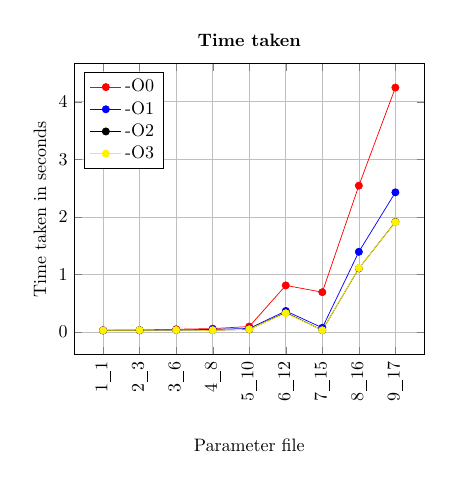
\begin{tikzpicture}[scale=0.65]
\begin{axis}[
	title={\textbf{Time taken}},
	ylabel={Time taken in seconds},
	%ymode=log,
	xlabel={Parameter file},
	x label style={yshift=-0.5cm},
	xtick={1,3,5,7,9,11,13,15,17},
	xticklabels={1_1, 2_3, 3_6, 4_8, 5_10, 6_12, 7_15, 8_16, 9_17},
	x tick label style={rotate=90, anchor=east},
	ymajorgrids=true,
	xmajorgrids=true,
	legend pos=north west,
	cycle list name=color list,
	]

\addplot+[mark=*] coordinates {
(1,0.031298) (3,0.032611) (5,0.050352) (7,0.061549) (9,0.097533) (11,0.811384) (13,0.693712) (15,2.54343) (17,4.24591)
};
\addlegendentry{-O0}

\addplot+[mark=*] coordinates {
(1,0.033393) (3,0.033572) (5,0.037248) (7,0.047957) (9,0.064181) (11,0.367553) (13,0.075426) (15,1.39464) (17,2.4274)};
\addlegendentry{-O1}

\addplot+[mark=*] coordinates {
(1,0.029873) (3,0.033931) (5,0.037498) (7,0.034361) (9,0.048934) (11,0.339495) (13,0.033142) (15,1.10833) (17,1.91377)};
\addlegendentry{-O2}

\addplot+[mark=*] coordinates {
(1,0.030431) (3,0.033729) (5,0.036896) (7,0.033898) (9,0.051484) (11,0.329233) (13,0.033632) (15,1.11276) (17,1.90869)};
\addlegendentry{-O3}

\end{axis}
\end{tikzpicture}
\end{minipage}
\caption{Optimisations with improved model on problem files \textit{with} solutions}
\end{figure}

\vspace{0.5cm}

\begin{figure}[H]
\centering
\begin{minipage}{0.45\textwidth}
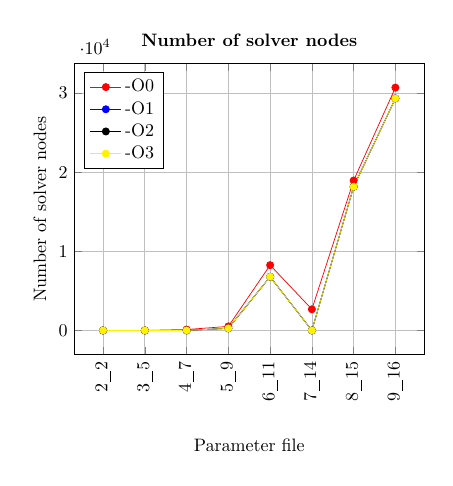
\begin{tikzpicture}[scale=0.65]
\begin{axis}[
	title={\textbf{Number of solver nodes}},
	ylabel={Number of solver nodes},
	%ymode=log,
	xlabel={Parameter file},
	x label style={yshift=-0.5cm},
	xtick={2,4,6,8,10,12,14,16},
	xticklabels={2_2,3_5,4_7,5_9,6_11,7_14,8_15,9_16},
	x tick label style={rotate=90, anchor=east},
	ymajorgrids=true,
	xmajorgrids=true,
	legend pos=north west,
	cycle list name=color list,
	]

\addplot+[mark=*] coordinates {
(2,0) (4,0) (6,113) (8,512) (10,8257) (12,2675) (14,18960) (16,30705) };
\addlegendentry{-O0}

\addplot+[mark=*] coordinates {
(2,0) (4,0) (6,0) (8,267) (10,6786) (12,0) (14,18169) (16,29331)};
\addlegendentry{-O1}

\addplot+[mark=*] coordinates {
(2,0) (4,0) (6,0) (8,267) (10,6786) (12,0) (14,18169) (16,29331)};
\addlegendentry{-O2}

\addplot+[mark=*] coordinates {
(2,0) (4,0) (6,0) (8,267) (10,6786) (12,0) (14,18169) (16,29331) };
\addlegendentry{-O3}

\end{axis}

\end{tikzpicture}
\end{minipage}
%
\begin{minipage}{0.45\textwidth}
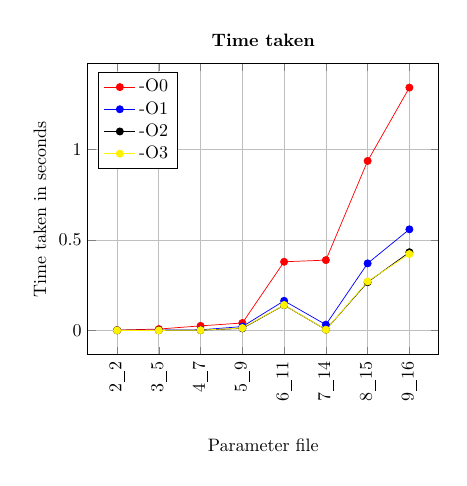
\begin{tikzpicture}[scale=0.65]
\begin{axis}[
	title={\textbf{Time taken}},
	ylabel={Time taken in seconds},
	%ymode=log,
	xlabel={Parameter file},
	x label style={yshift=-0.5cm},
	xtick={2,4,6,8,10,12,14,16},
	xticklabels={2_2,3_5,4_7,5_9,6_11,7_14,8_15,9_16},
	x tick label style={rotate=90, anchor=east},
	ymajorgrids=true,
	xmajorgrids=true,
	legend pos=north west,
	cycle list name=color list,
	]

\addplot+[mark=*] coordinates {
(2,0.001865) (4,0.007652) (6,0.025196) (8,0.041011) (10,0.379043) (12,0.388171) (14,0.93558) (16,1.34073)
};
\addlegendentry{-O0}

\addplot+[mark=*] coordinates {
(2,0.000863) (4,0.001497) (6,0.003385) (8,0.021171) (10,0.163485) (12,0.031769) (14,0.37022) (16,0.558146)};
\addlegendentry{-O1}

\addplot+[mark=*] coordinates {
(2,0.000551) (4,0.00099) (6,0.001367) (8,0.011141) (10,0.139455) (12,0.003976) (14,0.266379) (16,0.431757)};
\addlegendentry{-O2}

\addplot+[mark=*] coordinates {
(2,0.000111) (4,0.0) (6,0.001373) (8,0.013258) (10,0.140305) (12,0.004111) (14,0.270614) (16,0.421794)};
\addlegendentry{-O3}

\end{axis}
\end{tikzpicture}
\end{minipage}
\caption{Optimisations with improved model on problem files \textit{without} solutions}
\end{figure}


\end{appendices}



\printbibliography

\end{document}



